\documentclass{article}

\usepackage{graphicx} % Required for inserting images
\usepackage[left=1in,right=1in,top=1in,bottom=1in]{geometry} \usepackage{amsmath}
\usepackage{amsthm} %proof environment
\usepackage{amssymb}
\usepackage{amsfonts}
\usepackage{enumitem} %nice lists
\usepackage{verbatim} %useful for something 
\usepackage{xcolor}
\usepackage{setspace}
\usepackage{titlesec}
\usepackage{blindtext} % I have no idea what this is 
\usepackage{caption}  % need this for unnumbered captions/figures
\usepackage{natbib}
\usepackage{tikz}
\usepackage{hyperref}

\titleformat{\section}{\bfseries\Large}{Problem \thesection:}{5pt}{}
\titleformat{\subsection}{\bfseries\large}{Subproblem \thesubsection:}{5pt}{}

\begin{document}

\title{AM 160 - SciML:}
\author{Dante Buhl}


\newcommand{\wrms}{w_{\text{rms}}}
\newcommand{\bs}[1]{\boldsymbol{#1}}
\newcommand{\tb}[1]{\textbf{#1}}
\newcommand{\bmp}[1]{\begin{minipage}{#1\textwidth}}
\newcommand{\emp}{\end{minipage}}
\newcommand{\R}{\mathbb{R}}
\newcommand{\C}{\mathbb{C}}
\newcommand{\N}{\mathcal{N}}
\newcommand{\K}{\bs{\mathrm{K}}}
\newcommand{\m}{\bs{\mu}_*}
\newcommand{\s}{\bs{\Sigma}_*}
\newcommand{\dt}{\Delta t}
\newcommand{\dx}{\Delta x}
\newcommand{\tr}[1]{\text{Tr}(#1)}
\newcommand{\Tr}[1]{\text{Tr}(#1)}
\newcommand{\Div}{\nabla \cdot}
\renewcommand{\div}{\nabla \cdot}
\newcommand{\Curl}{\nabla \times}
\newcommand{\Grad}{\nabla}
\newcommand{\grad}{\nabla}
\newcommand{\grads}{\nabla_s}
\newcommand{\gradf}{\nabla_f}
\newcommand{\xs}{x_s}
\newcommand{\xf}{x_f}
\newcommand{\ts}{t_s}
\newcommand{\tf}{t_f}
\newcommand{\pt}{\partial t}
\newcommand{\pz}{\partial z}
\newcommand{\uvec}{\bs{u}}
\newcommand{\F}{\bs{F}}
\newcommand{\T}{\tilde{T}}
\newcommand{\ez}{\bs{e}_z}
\newcommand{\ex}{\bs{e}_x}
\newcommand{\ey}{\bs{e}_y}
\newcommand{\eo}{\bs{e}_{\bs{\Omega}}}
\newcommand{\ppt}[1]{\frac{\partial #1}{\partial t}}
\newcommand{\DDt}[1]{\frac{D #1}{D t}}
\newcommand{\ppts}[1]{\frac{\partial #1}{\partial t_s}}
\newcommand{\pptf}[1]{\frac{\partial #1}{\partial t_f}}
\newcommand{\ppz}[1]{\frac{\partial #1}{\partial z}}
\newcommand{\pp}[2]{\frac{\partial #1}{\partial #2}}
\newcommand{\dd}[2]{\frac{d #1}{d #2}}
\newcommand{\ddz}[1]{\frac{d #1}{d z}}
\newcommand{\ppzetas}[1]{\frac{\partial^2 #1}{\partial \zeta^2}}
\newcommand{\ppzs}[1]{\frac{\partial #1}{\partial z_s}}
\newcommand{\ppzf}[1]{\frac{\partial #1}{\partial z_f}}
\newcommand{\ppx}[1]{\frac{\partial #1}{\partial x}}
\newcommand{\ppxi}[1]{\frac{\partial #1}{\partial x_i}}
\newcommand{\ppxj}[1]{\frac{\partial #1}{\partial x_j}}
\newcommand{\ppy}[1]{\frac{\partial #1}{\partial y}}
\newcommand{\ppzeta}[1]{\frac{\partial #1}{\partial \zeta}}


\maketitle 
% This line removes the automatic indentation on new paragraphs
\setlength{\parindent}{0pt}
\doublespacing

\section{Learning the Lorenz' 96 Chaotic Attractor}

The lorenz' 96 system is given by the following dynamical system for $i,
j, k \in [1,8]$. 
\begin{gather*}
    \dd{X_i}{t} =
    X_{i-1}\left(X_{i+1}-X_{i-2}\right)-X_i + F -\frac{hc}{b}\sum_j Y_{i,j}\\
    \dd{Y_{i,j}}{t} =
    -cbY_{i,j-1}\left(X_{i,j+2}-Y_{i,j-1}\right)-cY_{i,j}+\frac{hc}{b}X_i-\frac{he}{d}\sum_k
    Z_{i,j,k}\\
    \dd{Z_{i,j,k}}{t} =
    edZ_{i,j,k-1}\left(Z_{i,j,k+1}-X_{i,j,k-2}\right)-geZ_{i,j,k}+\frac{he}{d}Y_{i,j}
\end{gather*}
Thus it is an 584-dimensional system (8 x variables, 64 y variables, and
512 z variables), and therfore its trajectories draw out a chaotic
attractor in 584-dimensional space. Sufficient parameters to create such
a system are $h = 0.5$, $c = 8$, $b = e = d = 10$, and $F = 20$. In this
assignment we will be ignoring the z variables completely (including the
dependence of the y variables on z), and evolving the system to see if
we can learn to predict the y variables using only the x positions as an
input. 

\begin{enumerate}[label = \alph*).]
    \item I will preface this by saying I have no idea what the procedure
    went over in class was and I don't use the published code to base my code.
    So I will hope that I am doing what the assignment describes and proceed to
    respond accordingly. The first task is to train a model to predict each of
    the 64 y variables using only the state of the x variables. This requires
    at the bare minimum that we have a model that takes in 8 inputs and
    after some variable number of hidden layers returns an output with 64
    outputs. I believe the entire context of how we train the network, what we
    use as a loss function, and everything else is variable and up to the
    student, because the assignment is very vague and doesn't describe any other
    constraints. 

    Thus I built a network and with I think 8 hidden layers and using the ReLU
    activation function between each layer. For training data, I used about 10-20 different
    trajectories of the Lorenz 96 system evolved from an RK4 integrator starting
    from initial conditions sampled from the the standard normal distribution.
    For each timeseries, about 10 epochs were used to train the model, and as a
    loss function, I chose the MSELoss function and specifically took the loss
    of the actual prediction error $|Y_{Act} - Y_{Pred}|$ and the loss of the
    term in the x equation $|\sum_{j} Y_{i,j, Act} - \sum_jY_{i,j, Pred}|$
    scaled up by 100 (so that it is more important than actually getting the y
    vector correct). 
    \begin{gather*}
        \text{Loss} = \left|\left|Y_{i,j,\text{Act}} -
        Y_{i,j,\text{Pred}}\right|\right|_2^2 +
        100\left|\left|\sum_j Y_{i,j,\text{Act}} - \sum_j Y_{i,j,\text{Pred}}\right|\right|_2^2
    \end{gather*}

    As shown in the output.txt file, using this method we are able to test the
    prediction error and find that the average error in $0.04$ for $Y$ and
    $0.81$ for $\sum_j Y_{i,k}$. 

    \item With $F = 24$, I am able to get relatively low prediction error. As
    shown in the output.txt file, the error obtained for $Y_{i,j}$ prediction is
    on average $0.05\ldots$ and the error obtained for $\sum_j Y_{i,j}$ is on average
    $1.02\ldots$. After training the model on the trajectory, the average loss
    is on the order of $0.039\ldots$ and $0.002\ldots$ respectively. 

    \item 

    \begin{figure}[ht]
        \centering
        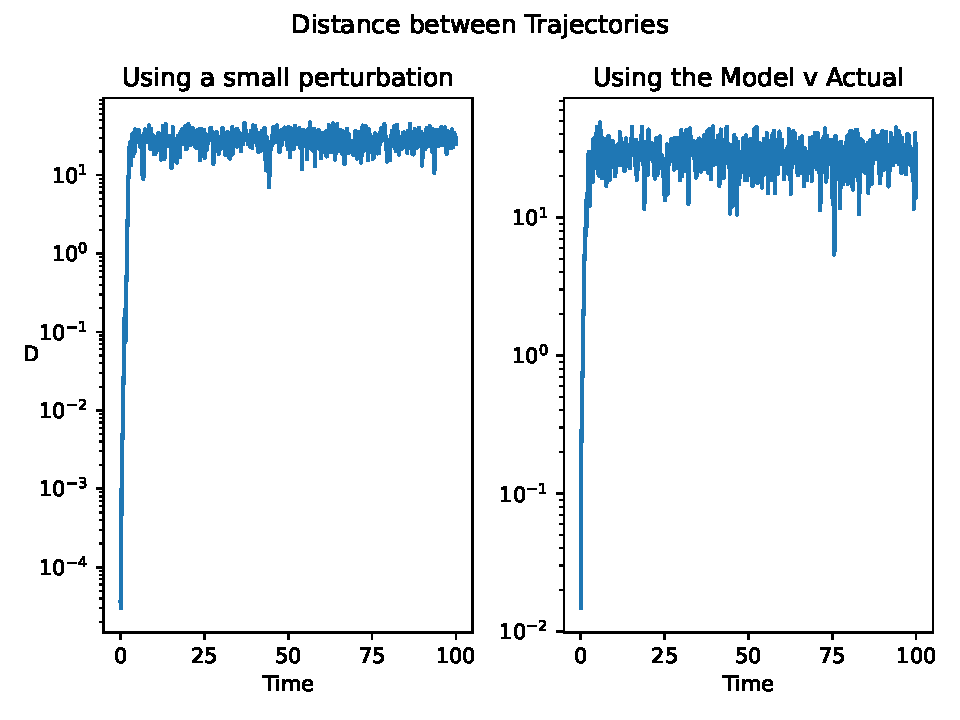
\includegraphics[width=\textwidth]{traj_div.pdf}
        \caption{Natural divergence between trajectories with infinitesimal
        perturbation using Lorenz96 (left) and divergence between trajectories
        with identical IC computed with
        Lorenz96M and Lorenz96 (right). Note that both stabilize to $O(10)$
        which indicates that the Lorenz96M system is able to recreate an attractor of the
        same general size (and hopefully shape), i.e. the model has successfully
        replicated the dynamics with a new lyapunov exponent.}
        \label{fig:attractor_size}
    \end{figure}

    Writing an RK4 integrator for this problem was very easy, the only
    change is that now the RK4 integrator evolves the Lorenz96M system where
    there are only 8 variables (the x variables) and furthermore, the model is
    introduced to make the x variables independent of $y$ and only need itself
    to evolve it time. That is, 
    \begin{gather*}
        \dd{X_i}{t} =X_{i-1}\left(X_{i+1}-X_{i-2}\right)-X_i + F
        -\frac{hc}{b}\sum_j M_{i,j}(\bs{X})
    \end{gather*}
    Note that this system is already stabilized at this point specifically
    for two reasons. First and foremost, the model is trained to primarily learn
    $S = \sum_j Y_{i,j}$ rather than $Y_{i,j}$ which is the pivotal point in
    reducing the complexity of the system. The next reason that this is
    stabilized is that by training on multiple trajectories which exist over
    long timeseries is that due to the chaotic nature of the system, the model
    has effectly (or rather hopefully) learned the attractor which the solution
    finds itself in. In order to demonstrate this, we show in Figure
    \ref{fig:attractor_size} that the model is able to predict $S$ within a
    reasonable level of accuracy which simply introduces a small error that
    grows in the system naturally over time. The key ingredient to this being a
    success is that the error in the Lorenz96M system stabilizes to the same
    error that the Lorenz96 system has for trajectories with small
    perturbations. In essence, we have learned the attractor. 


\end{enumerate}
\end{document}
